\section{The cross-correlation signal}
\label{sec:formalism}

The cross-correlation between a map of the UGRB, $\gamma(\hat{\bm n})$, and fluctuations in galaxy number counts, $g(\hat{\bm n})$, can be measured through the cross-correlation angular power spectrum (APS) \cite{camera2013novel,camera2015tomographic,fornengo2014particle}. In our analysis, the field $g$ will be the distribution of galaxies, which is a biased tracer of the underlying dark matter distribution. 
In the Limber approximation \citep{1953ApJ...117..134L,1992ApJ...388..272K,1998ApJ...498...26K}, the APS can be written as~{\cite{camera2013novel,camera2015tomographic,fornengo2014particle}}
\begin{equation}
 C_\ell^{\gamma g}=\int \frac{\de\chi}{\chi^2}\,\,W_{\gamma}(\chi)\, W_g(\chi)\,P_{\gamma g}\left(k=\ell/\chi,\chi\right)\;,
\label{eq:clfin}    
\end{equation}
%
 where $\ell$ denotes the multipole, $k$ the wavenumber, $\chi(z)$ is the radial comoving distance, related to redshift $z$ in a flat cosmology through the relation $\de\chi=c\,\de z/H(z)$ with $H(z)$ being the expansion rate of the Universe. The term $P_{\gamma g}(k,z)$ represents the 3D cross-correlation power spectrum (PS), embedding the information on the fluctuations of the two correlated fields. The function $W_{i=\{\gamma,g\}}$ denotes the window functions of the gamma-ray intensity field, $\gamma$, and the galaxy number counts fluctuations, $g$, {respectively, and describes the redshift distribution of each field} (see {\cref{app:model}} for full details).
 
As astrophysical $\gamma$-ray sources we consider only BL Lacs, subdivided into the two sub-categories of high-synchrotron-peaked (HSP) blazars and low and intermediate synchrotron-peaked (LISP) blazars \cite{DiMauro:2013zfa}.
We model the spectral energy distribution (SED) of these sources as power-laws with index $\varGamma$ and exponential cutoffs $E_\textrm{cut}$, whose specific parameter values are reported in \cref{table:BLLACS}, together with the minimum and maximum luminosities of the population.
Since we focus on CTAO and thus on energies above approximately {20} GeV, 
other typical $\gamma$-ray emitters like misaligned AGN, star-forming galaxies, and flat-spectrum radio quasars can be neglected, since their contribution are dominant at lower energies \cite{Fornasa_2015}. Full details on the modeling of the astrophysical sources are provided in {\cref{app:model}}, together with the expressions for their window functions and 3D cross-correlation power spectra, obtained within the halo model formalism.

Let us just recall here that the window function of the $\gamma$-ray emission of astrophysical sources depends on the $\gamma$-ray luminosity function (GLF) of each specific source-type and on their SED, and is integrated over the luminosity of the sources up to a threshold luminosity, which corresponds to the minimal luminosity that a source must posses in order to be resolved by the detector (in this way, the window function which is then obtained pertains to the \textit{unresolved} sources, those contributing to the UGRB). The full expression and the detailed modeling can be found in Appendix \ref{app:Wastro}.

For the DM $\gamma$-ray emission, we consider both annihilating and decaying DM. In the case of annihilation, the relevant particle physics parameters are the DM mass $m_\chi$ and the thermally-averaged annihilation cross-section $\langle \sigma v\rangle$. For decaying DM, the key parameters are the mass and the lifetime $\tau$. These will be the parameters for which we provide the forecast sensitivity in the cross-correlation analysis. The {expressions for the} window functions and the 3D cross-correlation power spectra are reported in {\cref{app:model}}. 
Here we recall that the window functions are proportional to $\langle \sigma v\rangle$ for annihilating DM and inversely proportional to $\tau$ in the case of decaying DM, and proportional to $m_\chi^{-2}$ and $m_\chi^{-1}$ for annihilating and decaying DM, respectively. The window function of the gamma-ray emission from DM annihilation or decay also depends on the average dark matter content of the Universe and on the energy spectrum produced by dark matter annihilation or decay, which in turn depends on the specific annihilation/decay channel, for which we will consider $b \bar b$ as the representative case and provide results also for the channels $e^+e^-$, $\tau^+\tau^-$ and $W^+W^-$. In the case of annihilating dark matter, the window function also contains a so-called flux-multiplier factor, which accounts for the enhancement of the flux due to the clumping of DM and the presence of sub-structures within the DM halos. The full expressions and the detailed modeling of the DM window functions can be found in Appendix \ref{app:WDM}. A few examples of the redshift behavior of the $\gamma$-ray window functions for DM annihilation are shown in Fig. \ref{fig:window_main}, for two photon energies and two DM masses. For comparison, we also show the window functions of unresolved LISP and HSP astrophysical source classes, assuming an observation time of 3 hours. The observation time affects the window functions of astrophysical sources, since it determines the minimum luminosity of the sources that can be resolved by the instrument (and therefore do not contribute to the unresolved component consider in our analysis). The case for 50 hours of observation is shown in Fig. \ref{fig:zWindows} in {\cref{app:model}}.

\begin{figure}[t!]
    \centering
    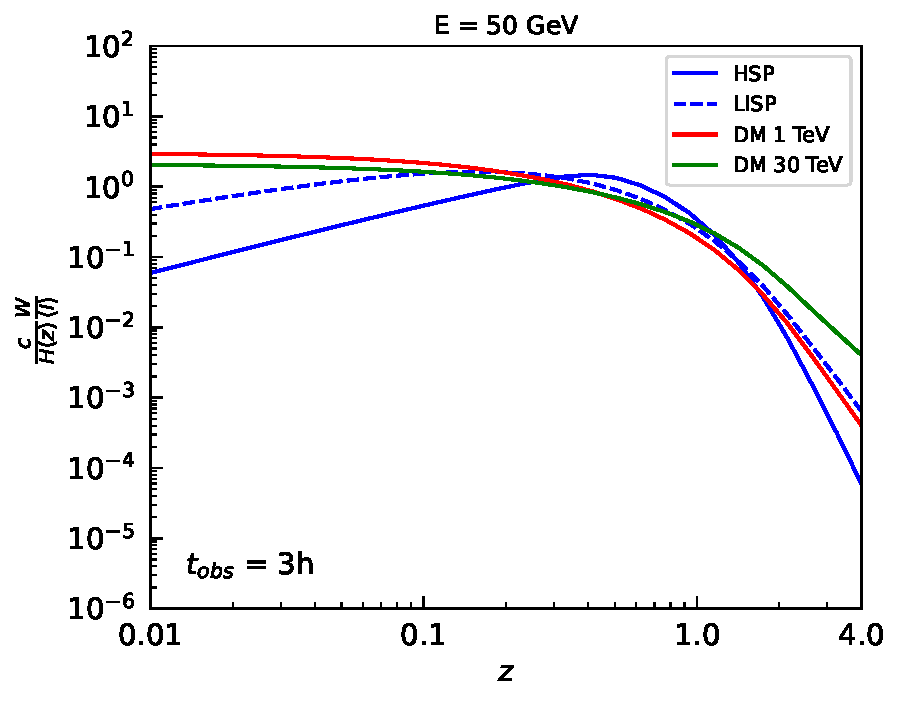
\includegraphics[width=0.45\textwidth]{figures/new_analysis/W_at_50GeV_3h.pdf}
    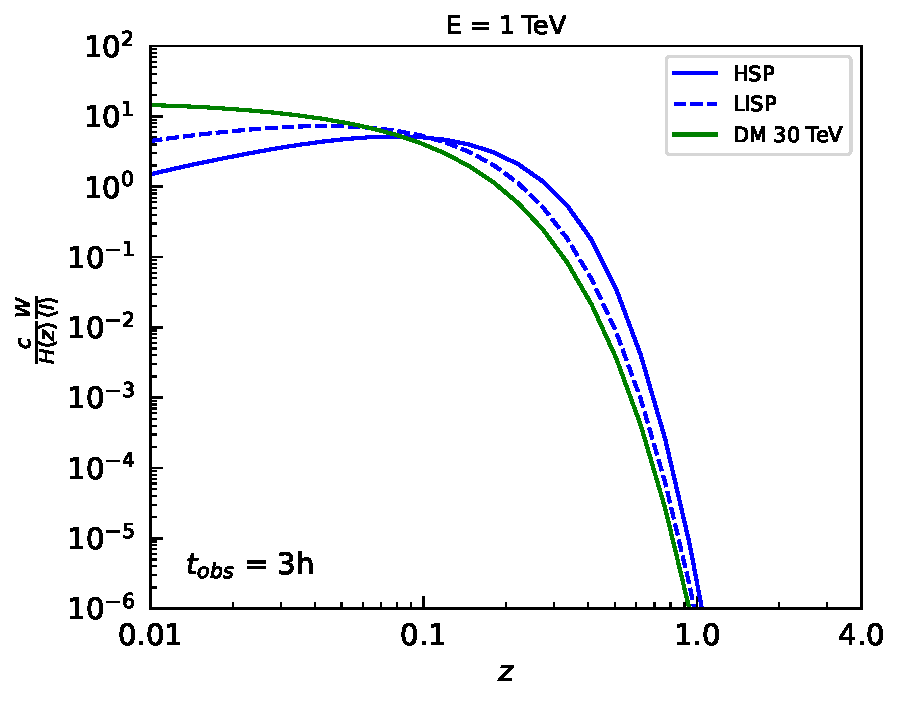
\includegraphics[width=0.45\textwidth]{figures/new_analysis/W_at_1TeV_3h.pdf}
    \caption{The $\gamma$-ray window functions, normalized to the mean $\gamma$-ray intensity and divided by the Hubble parameter, as a function of redshift. Blue solid and dashed lines show HSP and LISP astrophysical sources for 3 hours of observation, respectively. Red and green lines correspond to DM annihilation into $b\bar{b}$, $\langle \sigma v \rangle = 3 \times 10^{-26}$cm$^{-3}$s$^{-1}$ for DM masses of 1 TeV (red) and 30 TeV (green). Upper panel: $E_\gamma = 50$ GeV; lower panel: $E_\gamma = 1$ TeV (only 30 TeV DM case shown).}
    \label{fig:window_main}
\end{figure}

For the present analysis, which primarily focuses on the sensitivity to a DM signal, we adopt as galaxy catalogs the Two Micron All-Sky Survey (2MASS) \cite{2MASS:2006qir,Bilicki:2013sza} and the 2MASS Redshift Survey (2MRS) \cite{Huchra:2011ii,Ando:2017wff} catalogs, since they cover the low redshift range $z \lesssim 0.1$ where most of the DM $\gamma$-ray emission originates.
Astrophysical sources, on the other hand, have a peak in emission at redshifts $z\sim 0.3$--$0.4$ at $E\sim {50}\,\textrm{GeV}$, and $z\sim 0.1$--$0.2$ at $E\gtrsim 1\,\textrm{TeV}$
as shown {in Fig. \ref{fig:window_main} and in Fig. \ref{fig:zWindows}} in {\cref{app:model}}.
The latter range is a consequence of strong absorption of $\gamma$-rays above $\sim 1 \textrm{TeV}$ due to interactions with the extragalactic background light (EBL), which limits the $\gamma$-ray horizon to $z\sim 0.1$--$0.2$ independently of the type of source.

The present analysis is thus optimized for DM searches, while for astrophysical sources it will be beneficial to consider galaxy catalogs covering higher redshifts, up to $z\sim 0.4-0.5$. We leave this extension to future studies. The window functions of galaxy number counts are given by the redshift distribution of the number of objects in the catalog. Full details on the window functions of the catalogs adopted here can be found in {\cref{app:Wgal}}. The modeling of galaxy clustering within halos is based on the halo occupation distribution (HOD) formalism~\cite{Zheng:2004id,Berlind:2001xk,Cooray:2002dia}, which is also outlined in {\cref{app:model}}, together with the 3D cross-correlation power spectra. 

Let us note that in our analysis, the window function $W_g(z)$ of the galaxy catalogs is normalized to unity: $\int \de z\, W_g(z) =1$. For the $\gamma$-ray window function $W_\gamma(\chi)$, we define it such that the (average) intensity energy spectrum is obtained as: $I_{\gamma}(E) = \int \de\chi\ W_\gamma(E,\chi)$. 

The cross-correlation APS signal has a variance $\smash{(\varDelta C^{\gamma g}_\ell)^2}$ given by~{\cite{camera2013novel,camera2015tomographic,fornengo2014particle}}
\begin{multline}
    (\varDelta C^{\gamma g}_\ell)^2 \,(2\,\ell+1)\,f_\textrm{sky} =  \\ (C_\ell^{\gamma g})^2 + \left[C_\ell^{\gamma \gamma} + \frac{C_N}{(B_\ell)^2}\right]\,\left(C_\ell^{gg} + C_{N_g} \right)\;, \label{eq:Delta}
\end{multline}
where $C_\ell^{\gamma\gamma}$ and $C_\ell^{gg}$ are the $\gamma$-ray and galaxy auto-correlation APS, $C_N$ is the photon noise, $C_{N_g}$ the galaxy catalog noise, and $B_\ell$ denotes the beam correction {accounting for the finite angular resolution of the $\gamma$-ray instrument. No beam correction is applied to the galaxy term, since the angular resolution of galaxy catalogs (typically of the order of arcseconds) is negligible for the purposes of this analysis. The parameter} $f_\textrm{{sky}}$ denotes the fraction of the sky covered by the analysis. All the relevant terms in \cref{eq:Delta} are outlined in {\cref{app:model}}.

For completeness, in the following analysis, we will also use the $\gamma$-ray auto-correlation APS, which is a measure of the intrinsic anisotropy of the $\gamma$-ray emission. It reads~\cite{Ando:2013ff,camera2013novel,camera2015tomographic,fornengo2014particle}
\begin{equation}
 C_\ell^{\gamma \gamma}=\int \frac{\de\chi}{\chi^2}\,W_{\gamma}^2(\chi)  
 \,P_{\gamma \gamma}\left(k=\ell/\chi,\chi\right)\;,
\label{eq:clfin_auto}    
\end{equation}
where $P_{\gamma \gamma}$ is the 3D power spectrum of the $\gamma$-ray emission. The corresponding variance on $C_\ell^{\gamma \gamma}$ is~{\cite{camera2013novel,camera2015tomographic,fornengo2014particle}}
\be
(\varDelta C_\ell^{\gamma \gamma})^2 = \frac{2}{(2\,\ell+1)\,f_\textrm{sky}} \left[C_\ell^{\gamma \gamma} + \frac{C_N}{(B_\ell)^2} \right]^2\;.\label{eq:variance_gammagamma}
\ee


\begin{table}[t!]
\centering
\begin{tabular}{|m{0.07\textwidth} |m{0.06\textwidth} m{0.12\textwidth} m{0.10\textwidth} m{0.10\textwidth}|} 
\hline
  & $\varGamma$ & $E_{\text{cut}}$ [GeV] & $L_\textrm{min}$ [erg/s] & $L_\textrm{max}$ [erg/s]  \\ [0.5ex]
 \hline
 HSP & 1.86 & 910 $^{+1100}_{-450}$ & $10^{38}$ & $3\cdot 10^{45}$  \\ [0.5ex]
 LISP & 2.08 & 37 $^{+85}_{-20}$ & $10^{38}$ & $3\cdot 10^{46}$ \\ [1ex]
 \hline 
\end{tabular}
\caption{Parameters and uncertainties for the power-law with exponential cut-off SED models of HSP and LISP populations, including the minimum and maximum luminosity, adopted from Table 1 of Ref. \cite{DiMauro:2013zfa}.}
\label{table:BLLACS}
\end{table}

%%%%%%%%%%%%%%

